\chapter{Implementation}
\thispagestyle{main} % Needed for Footer and Header on Chapterpage
This chapter focuses on explaining why things were implemented in a certain manner. Here the trade-offs and decisions which were taken while building the VM are described in a manner that follow up works get a better understanding of why some parts of the VM are implemented in a certain way so that they either are more certain when changing something or to help them reach the same conclusion faster.

\begin{figure}[H]
	\begin{center}
	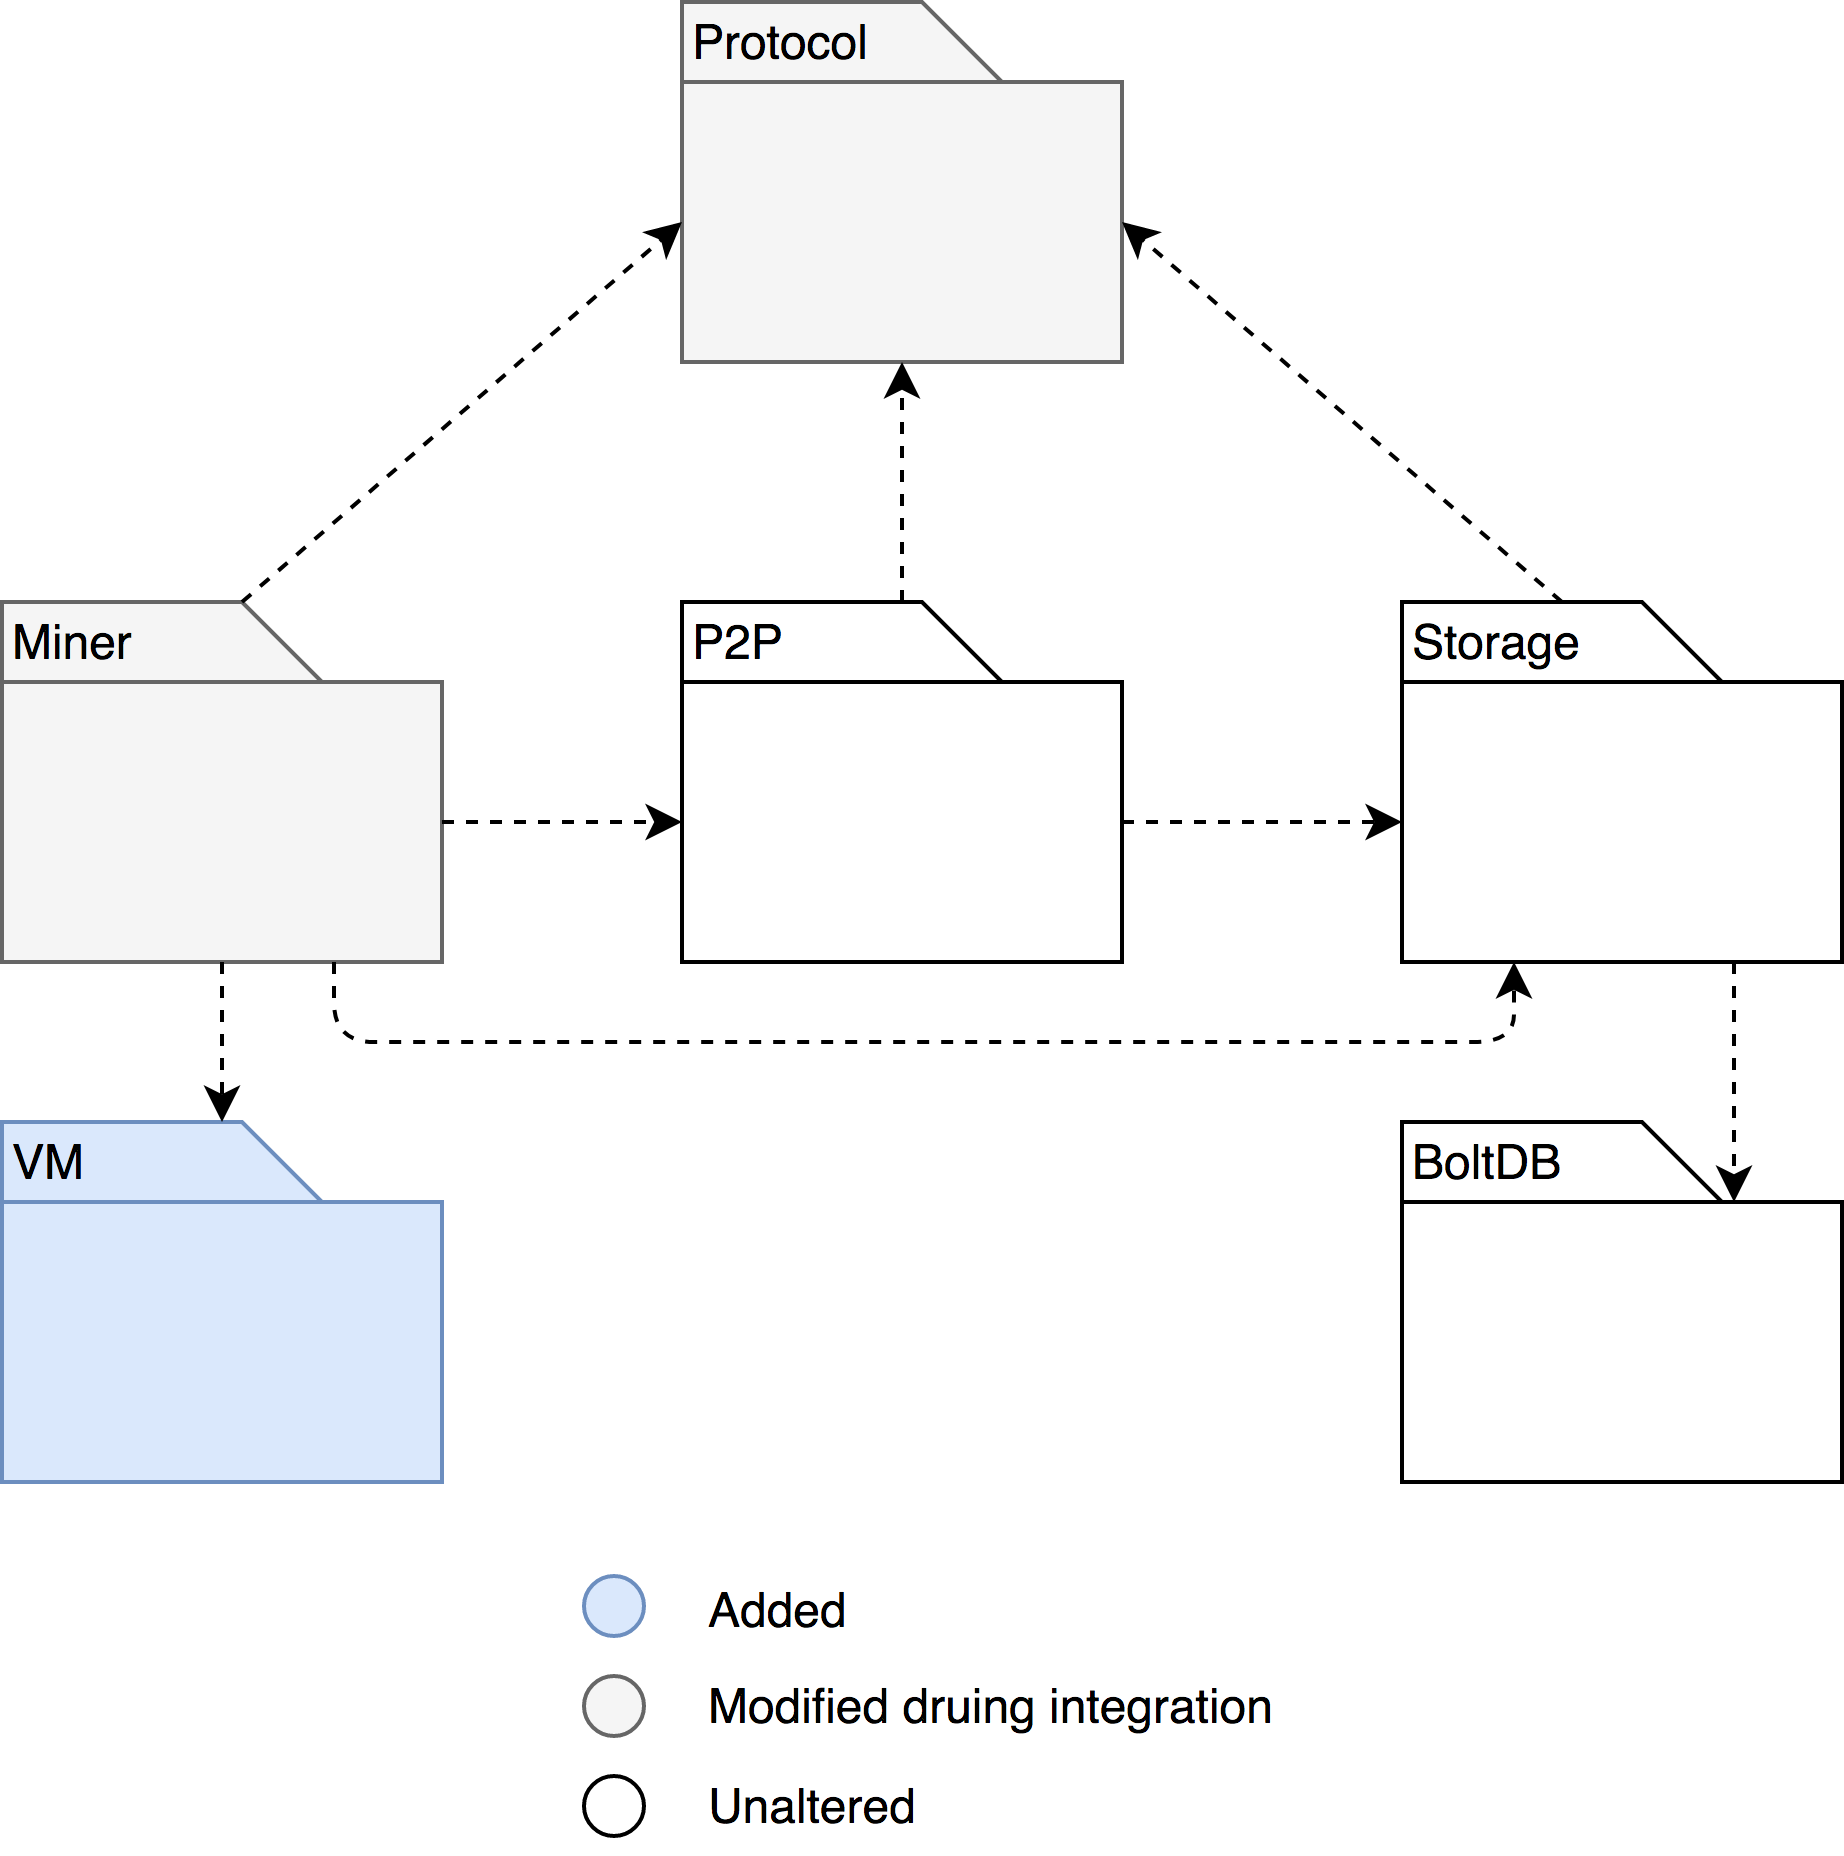
\includegraphics[width=0.7\textwidth]{./images/package-diagram}
	\caption{UML Package Diagram}
	\label{package overview}
	\end{center}
  \end{figure}

\section{Contract execution}

\section{VM Package overview}
As the miner and all other projects are written in golang, for this project also golang is used.
At the time of writing this thesis the VM consists of the following classes:
% Insert execution cycle graphic

\section{Stack}

% TODO insert crc card for stack

\subsection{Maximum stack size}
Facing the concern of excess memory usage of the contract on the miner, we decided to limit the stack size to 1MB which seems to be well above what the contracts will need. We neglected using the gas amount for max storage determination because it would be just a soft limit

\subsection{Maximum variable size}
Since it is possible to easily craft denial of service attacks for the blockchain if there is no limit on the variable size we decided to set the variable size to a specific fixed amount instead of arbitrary precision.

\subsection{Data structure}
As underlying data structure of "Stack", keeping in mind to keep the code of the vm short and simple, we decided to use an array of big.Int. It was important that the datatype used for the underlying datatype was of arbitrary length because splitting up an element into multiple bytes so that it can be saved when using an array of bytes as underlying data structure would have been a lot more complex and more error-prone. Arbitrary length is implemented for example an array of jagged arrays of bytes. On the vm it was very important that the type used in the vm provided mathematical methods and also that it could store and work with values of up to 256 bit size. Only big.Int fulfilled both requirements and therefore it was choosen for the vm. Thanks to big.Int being of arbitrary length we could then use an array of big.Int as underlying data structure which also simplifies our code since we don't have to cast the values retrieved from the stack before working with them.

We neglected working with pointers because even though there are more elements created on the heap of the physical machine, it shouldn't make a difference considering the vast availability of resources on modern computers and our rather small contracts. We neglected using a simple array of bytes as the whole data structure where different datatypes are read using a different amount of bytes, as it is common when having no abstraction layer or using a jagged array of byte arrays because the could becomes a lot more readable in the vm and less conversions from big.Int to byte array are necessary. We accept the dependency on the datatype big.Int which is necessary as it implements all mathematical operations which are very important and because it is of arbitrary precision and the size of other datatypes would not have been sufficient especially for cryptographic purposes.

\section{Virtual machine}
The virtual machine itself is implemented as a switch case where it takes different bytes and determines what has to be executed on each value.

% TODO insert crc card for vm
\subsection{opCodes}
% Please add the following required packages to your document preamble:
% \usepackage{booktabs}
\begin{table}[]
\centering
\caption{List of opCodes available}
\label{opcodes-list}
\begin{tabular}{@{}llll@{}}
\toprule
\textbf{Instruction} & \textbf{Mnemonic} & \textbf{opCode} & \textbf{Description}                                     \\ \midrule
Push Bytes           & PUSH              & 0x00            & stack $\leftarrow$ bytes                                            \\
Duplicate            & DUP               & 0x01            & stack $\leftarrow$ peek1                           \\
Roll                 & ROLL              & 0x02            & removes element at index and push to ToS           \\
Pop                  & POP               & 0x03            & pops ToS                                                 \\
Add                  & ADD               & 0x04            & stack $\leftarrow$ pop1 \+ pop2                                      \\
Subtract             & SUB               & 0x05            & stack $\leftarrow$ pop1 \- pop2                                      \\
Multiply             & MULT              & 0x06            & stack $\leftarrow$ pop1 \* pop2                                      \\
Divide               & DIV               & 0x07            & stack $\leftarrow$ pop1 \/ pop2                                      \\
Modulo               & MOD               & 0x08            & stack $\leftarrow$ pop1 \% pop2                                     \\
Negate               & NEG               & 0x09            & stack $\leftarrow$ todo                                             \\
Equals               & EQ                & 0x0a            & stack $\leftarrow$ 1 if pop1 == pop2, 0 otherwise                   \\
Not equal            & NEQ               & 0x0b            & stack $\leftarrow$ 1 if pop1 != pop2, 0 otherwise                   \\
Lower than           & LT                & 0x0c            & stack $\leftarrow$ 1 if pop1 \textless{} pop2, 0 otherwise            \\
Greater than         & GT                & 0x0d            & stack $\leftarrow$ 1 if pop1 \textgreater{} pop2, 0 otherwise         \\
Lower than/equals    & LTE               & 0x0e            & stack $\leftarrow$ 1 if pop1 \textless{}= pop2, 0 otherwise         \\
Greater than/equals  & GTE               & 0x0f            & stack $\leftarrow$ 1 if pop1 \textgreater{}= pop2, 0 otherwise      \\
Shift left           & SHIFTL            & 0x10            & stack $\leftarrow$ pop 1 \textless{}\textless nrOfShifts            \\
Shift right          & SHIFTR            & 0x11            & stack $\leftarrow$ pop 1 \textgreater{}\textgreater nrOfShifts      \\
No operation         & NOP               & 0x12            & does nothing                                             \\
Jump                 & JMP               & 0x13            & jump to address                                          \\
Jump if true         & JMPIF             & 0x14            & jumps to address if pop1 == 1                            \\
Call                 & CALL              & 0x15            & call a function                                          \\
Call if true         & CALLIF            & 0x16            & calls a function if pop1 == 1                            \\
Call external        & CALLEXT           & 0x17            & calls function from external smart contract              \\
Return               & RET               & 0x18            & returns from function                                    \\
Size of ToS          & SIZE              & 0x19            & stack $\leftarrow$ size(pop1)                                       \\
Store                & STORE             & 0x1a            & stores pop1 in callStack                                 \\
State Store          & SSTORE            & 0x1b            & stores pop1 in contractVariables                         \\
Load                 & LOAD              & 0x1c            & stack $\leftarrow$ var from callStack
    \\
State Load           & SLOAD             & 0x1d            & stack $\leftarrow$ receiver var from contractVariables \\
Address              & ADDRESS           & 0x1e            & stack $\leftarrow$ receiver account address                         \\
Balance              & BALANCE           & 0x1f            & stack $\leftarrow$ receiver account balance                         \\
Caller               & CALLER            & 0x20            & stack $\leftarrow$ contract caller                                  \\
Call value           & CALLVAL           & 0x21            & stack $\leftarrow$ transaction amount in bazo coins                 \\
Call data            & CALLDATA          & 0x22            & stack $\leftarrow$ transaction data                                 \\
New map              & NEWMAP            & 0x23            & stack $\leftarrow$ new map                                          \\
Map push             & MAPPUSH           & 0x24            & stack $\leftarrow$ add entry to map                                 \\
Map get value        & MAPGETVAL         & 0x25            & todo                                                     \\
Map set value        & MAPSETVAL         & 0x26            & todo                                                     \\
Map remove           & MAPREMOVE         & 0x27            & todo                                                     \\
New array            & NEWARR            & 0x28            & stack $\leftarrow$ new array                                        \\
Array append         & ARRAPPEND         & 0x29            & todo                                                     \\
Array insert         & ARRINSERT         & 0x2a            & todo                                                     \\
Array remove         & ARRREMOVE         & 0x2b            & todo                                                     \\
Array index at       & ARRAT             & 0x2c            & todo                                                     \\
SHA3 Hashing         & SHA3              & 0x2d            & stack $\leftarrow$ SHA3\_HASH(pop 1)                                \\
Check signature      & CHECKSIG          & 0x2e            & todo                                                     \\
Halt with error      & ERRHALT           & 0x2f            & return from Exec() function with false                   \\
Halt                 & HALT              & 0x30            & return from Exec() function with true                    \\ \bottomrule
\end{tabular}
\end{table}

\subsection{call stack}

\subsubsection{Datastructures}
describe the implementation of map, array and how one could create a struct. Do it the same as the other opcodes.

\subsection{Context}

\subsection{Sideffects on data}

Since the VM operates on copies the values will also not be changed by a faulty contract.

\section{Integration}

\subsection{Testing}
\subsubsection{Test Driven Development}
The project was implemented with test driven development. 

\subsubsection{Fuzz Testing}
An instruction in a smart contract must never be able to crash the miner. Calling a smart contract function with malicious instructions would cause the whole blockchain to collapse. To check if the VM fails gracefully, a fuzz test was implemented which creates contracts with real random bytes and then executes them. Contracts causing the miner to crash were reproduced as unit test in order to find the bug. Once the bug was fixed it was mitigated. This process was repeated over and over again. Starting the fuzz test with five million random contracts with every commit to the remote repository and having run it with a billion random contracts over night makes us confident that every bug was found and mitigated.

\subsection{Error handling}
The VM just processes one operation code after the other.

One of the problems is that it is possible to write byte code which is not possible for the vm to execute, for example byte code which tells the vm to push six bytes on the stack when there is only one byte left in the byte code. This of course means that an error occurs somewhere in the vm. In this example of course when trying to fetch the next arguments. It was paid a lot of attention to put guards around such critical sections to avoid calling these with invalid values and define graceful failures with error object  the message of which is later on pushed on the stack of the vm. After that the vm halts.

%insert number of testcoverage

\section{Parser}
